\section{Simulation Analysis}
\label{sec:simulation}

In this section, the intent is to simulate the circuit, using \textit{Ngspice}.

Firstly, the AC/DC converter was subjected to a transient simulation. Then the outputs of the envelope detector and voltage regulator circuits were plotted as shown in the following figures \ref{plot5} and \ref{plot6}, along with the output $v_4(t)-12V$ (DC deviation with the AC component) plot in Figure \ref{plot7}. 

\begin{figure}[h]
    \centering
    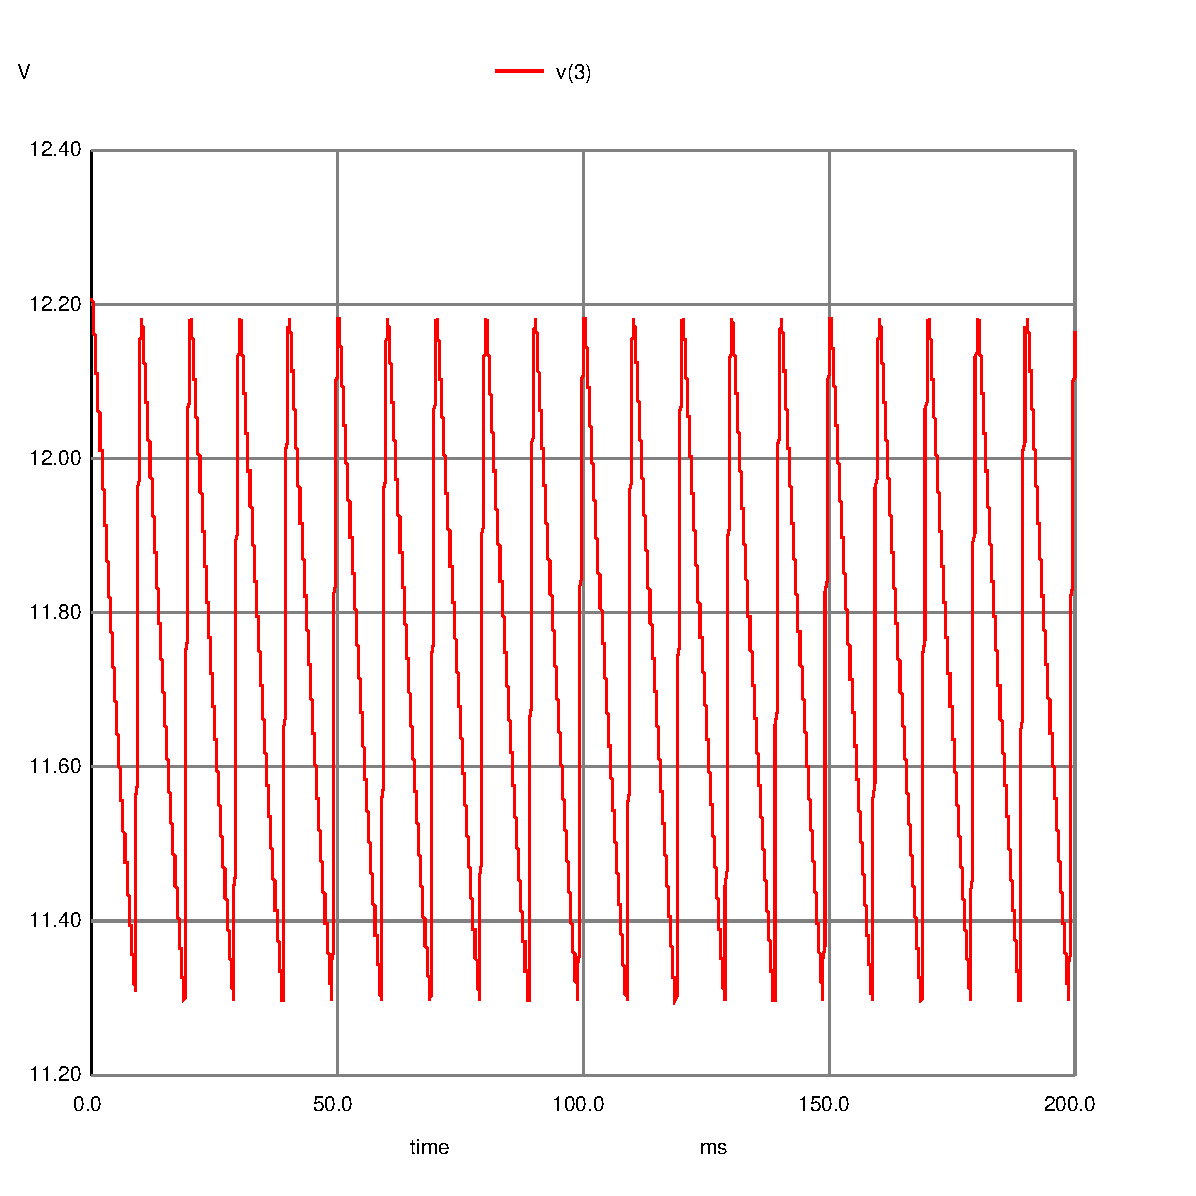
\includegraphics[width=0.6\linewidth]{v_3.eps}
    \caption{Voltage after the envelope detector}
    \label{plot5}
\end{figure}

\begin{figure}[h]
    \centering
    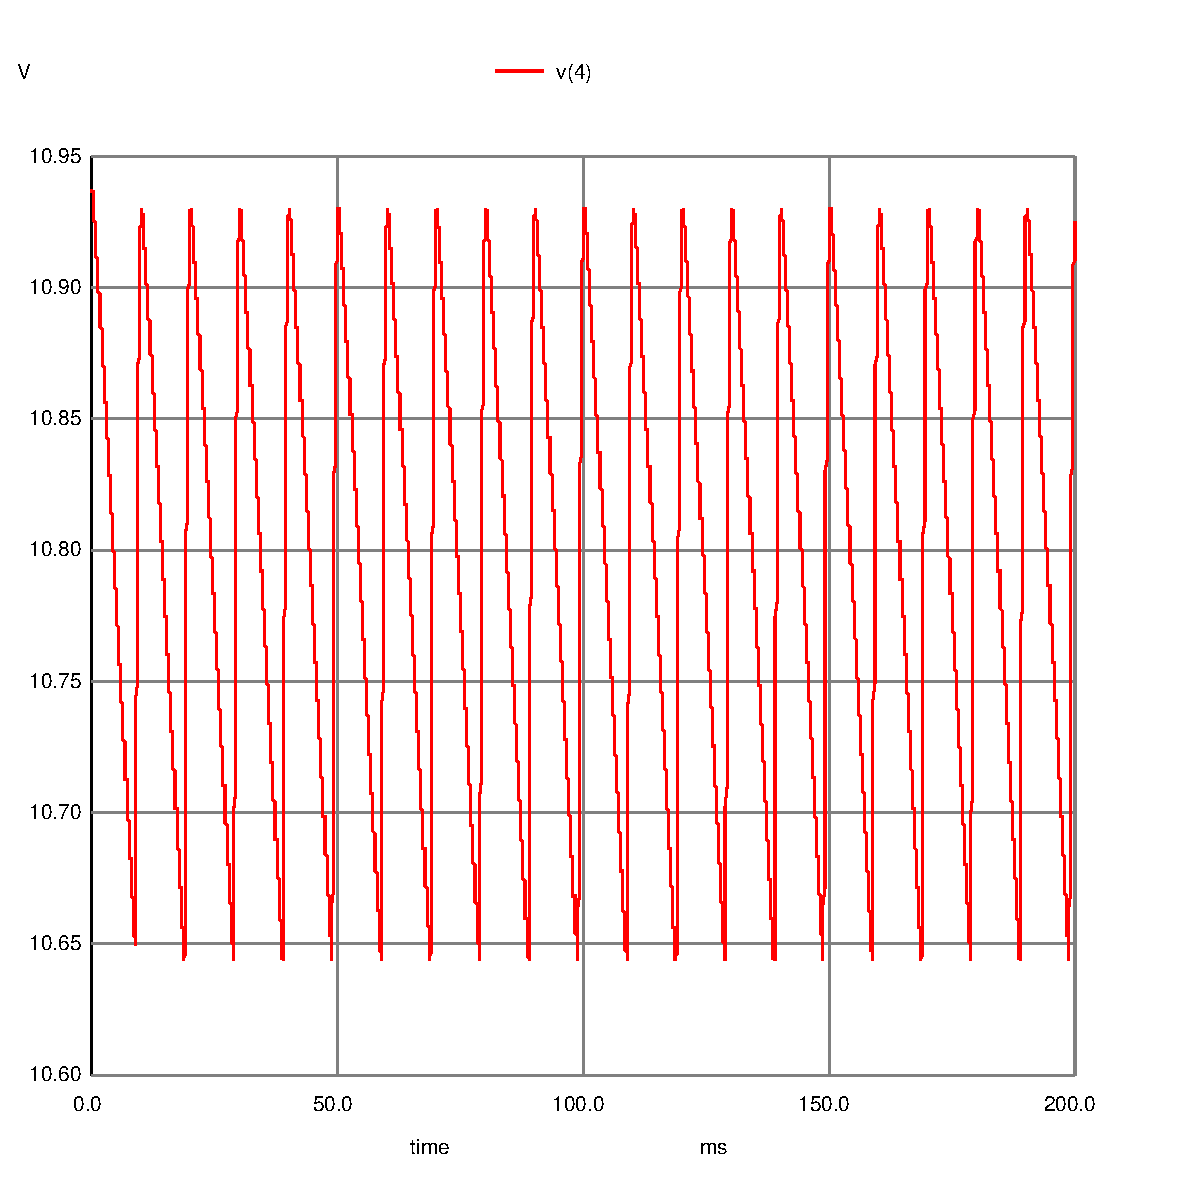
\includegraphics[width=0.6\linewidth]{v_4.eps}
    \caption{Voltage after the regulator}
    \label{plot6}
\end{figure}

\begin{figure}[h]
\centering
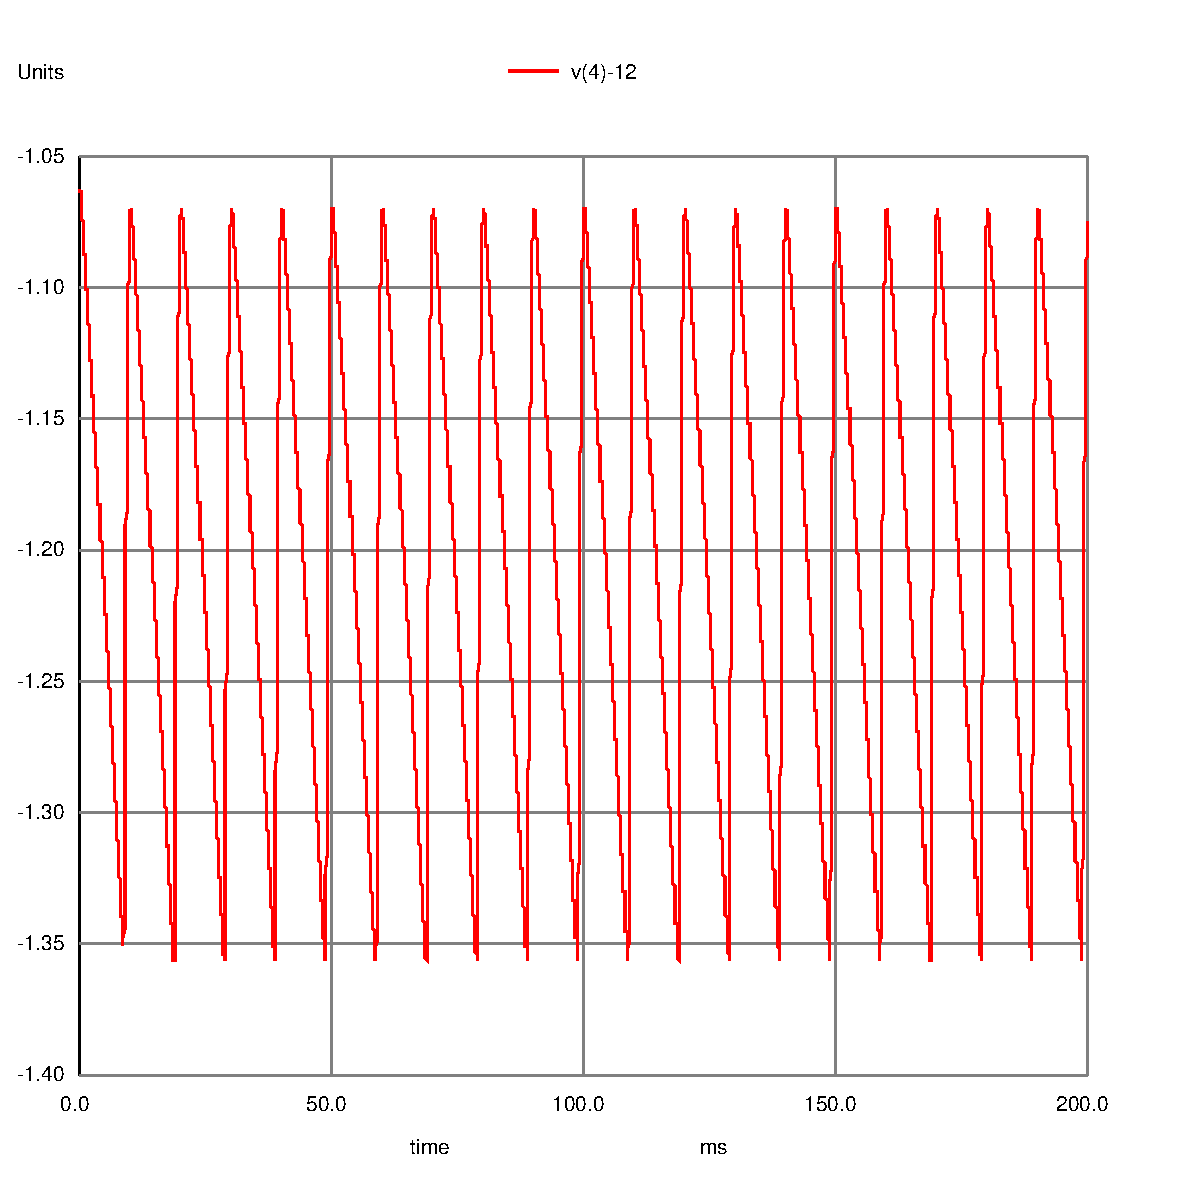
\includegraphics[width=0.6\linewidth]{delta_v.eps}
\caption{Voltage difference between the regulator output and the 12 V DC}
\label{plot7}
\end{figure}

\clearpage

The output voltage ripple and the DC level were simulated aswell and are as follows.

\begin{equation}
    V_{Ripple} = 0.2933 V
\end{equation}
\begin{equation}
    DC Level = 10.798
\end{equation}


\subsection{Comparisons}
\label{subsec:compare}

%In this last subsection, we present the values and plots obtained from the Theoretical Analysis and the Simulation Analysis that refer to the same sets of evaluations, for visualization purposes, and comment on their similarities or discrepancies.



All in all, there is an obvious difference between the theoretical and simulation results. The results obtained using \textit{Octave} are closer to the aimed values and oscillate less. The values obtained with \textit{Ngspice} are smaller ($v_4(t)$ is closer to 11V, for example). Nevertheless, the overall wave forms are similar, the frequency of the signals is the same, and, by both approaches, the results are satisfyingly accurate. 
The discrepancies stem from the different considerations made in the theoretical model and in the Ngspice software's models. In the Ngspice models, the approximations used when diodes are involved are much more complex and accurate.
